\documentclass{article}
\usepackage[T1]{fontenc}
\usepackage[utf8]{inputenc}
\usepackage{microtype}
\usepackage{graphicx}
\usepackage{booktabs,tabularx,multirow,array}
\usepackage{amsmath,amssymb,amsthm,mathtools}
\usepackage{xcolor}
\usepackage{xurl}
\usepackage{hyperref}
\usepackage{mlsys2025}
\usepackage{enumitem}
\newcommand{\famp}{\textsc{Famp}}
\newcommand{\E}{\mathbb{E}}
\newcommand{\R}{\mathbb{R}}
\newcommand{\ind}{\mathbf{1}}
\newcommand{\bytes}{\operatorname{bytes}}
\newcommand{\risk}{\mathcal{R}}
\newcommand{\blank}{\phantom{00.00}}
\newcommand{\RQ}[1]{\textbf{RQ#1}}
\newcommand{\code}[1]{\texttt{\small #1}}
\newtheorem{proposition}{Proposition}
\newtheorem{definition}{Definition}
\newcolumntype{Y}{>{\raggedright\arraybackslash}X}
\hypersetup{pdfauthor={Anonymous authors},pdfsubject={Research draft; confirmatory tables intentionally empty}}
\mlsystitlerunning{FAMP: Executable Memory for Byte-Budgeted Continual Learning}

\mlsystitlerunning{FAMP: Supplementary Protocol and Artifact Specification}
\renewcommand{\thetable}{A\arabic{table}}
\renewcommand{\thefigure}{A\arabic{figure}}
\renewcommand{\theequation}{A\arabic{equation}}
\begin{document}
\twocolumn[
\mlsystitle{FAMP: Supplementary Protocol, Guarantees,\\and Artifact Specification}
\begin{mlsysauthorlist}\mlsysauthor{Anonymous Authors}{anon}\end{mlsysauthorlist}
\mlsysaffiliation{anon}{Anonymous Institution}
\mlsyscorrespondingauthor{Anonymous Author}{anonymous@example.com}
\vskip .3in]
\printAffiliationsAndNotice{}
\noindent\textbf{Companion status.} This appendix is a separate upload, not an extension of the main-paper page allowance. It fixes operational details, data access, baseline obligations, and table definitions. Numerical result cells remain empty. The executed development pilot, checkpoints, and generated insights are separate artifacts; they do not stand in for the confirmatory image, modular-baseline, or multi-device experiments.
\appendix

\section{Exact System Specification}
\label{app:system}
\subsection{Published and temporary objects}
A published learner contains a mutable fallback network, a list of frozen unit state dictionaries, a map from task identifiers to frozen readout heads and unit IDs, bounded witness packets, residual replay arrays, and canonical metadata. The public schema identifier binds these objects to a fixed implementation. The configuration and source digest accompany the checkpoint archive. Public code and common executable libraries are not charged as learned task memory; all task-specific tensors and route metadata are. Container file headers are reported separately from the payload ledger.

The published-state metric counts tensor elements times their actual storage widths and the UTF-8 length of canonical JSON. For replay, input arrays, labels, task IDs, priorities, and any retained logits are counted. For each witness packet, stored inputs, labels, teacher probability targets, and perturbation seeds are counted. A physical unit appears once in the bank regardless of how many routes reference it. Every referencing head and its identifier list is still counted. No trained feature cache is retained at inference.

Adam moments, gradients, task-local candidate parameters, cached features for fitting heads, and temporary packed/depacked tensors are workspace. They are real resource costs but not silently included or excluded by renaming them ``knowledge.'' The main persistent-cap claim is restricted to published boundaries. In the artifact, observer datasets may reside in the same Python process for reproducibility; a process-RAM claim must use isolated learner profiling or explicitly include that observer footprint. The supplied CPU pilot does not certify peak process RAM, GPU energy, or production throughput.

\subsection{Inference semantics}
For a covered task, the learner evaluates its referenced units on raw preprocessed inputs, concatenates their outputs, and evaluates its frozen linear head. Task identity selects the route directly. No trainable preprocessing, shared normalization statistics, mutable embedding, or fallback feature tensor lies upstream of an admitted route. For an uncovered task, the fallback receives raw input and a task one-hot vector concatenated \emph{before} two nonlinear layers. This allows different task-specific decision functions, not only task-specific biases.

Synthetic and Digits tasks use two output classes. CIFAR task IDs identify ten-way class subsets, and local labels are mapped from global class IDs. Evaluation never presents the local task head as a 100-way class-incremental classifier. Requiring task identity is an information advantage relative to task-agnostic learning and must be matched in any baseline comparison.

\subsection{Candidate construction}
Each stage first trains the fallback on current-task examples and available replay. The current fallback is then held fixed while candidates are built. Existing unit candidates train only a linear head on cached, frozen features. The composition candidate concatenates two existing units. A new unit is trained with current labels plus temperature-two teacher distillation and then receives a separately fitted candidate head. The discarded training head and teacher outputs are workspace, not retained memory.

The shortlist contains the last three admitted units, not the three tasks most similar under an oracle. The composition proposal uses the last two shortlist entries. With a full shortlist, at most five proposals are considered: three singleton reuses, one composition, and one allocation. This bounded policy is intentionally simple. It is not an exhaustive search over all subsets, and the implementation does not infer a variable number of semantic primitives.

Selection uses a separate split. Eligible candidates are within six percentage points of selection teacher accuracy in the pilot. Among them, the policy minimizes incremental \emph{parameter} bytes; it breaks ties using selection accuracy. All witness and metadata bytes are subsequently included in the transaction. The local proxy can therefore propose a route that later fails the true byte cap. A rejection is recorded, rather than retried with a second candidate on the same acceptance set. Such a retry would require an additional statistical correction or new data.

\subsection{Persistent-state transaction}
An accepted candidate stages a new unit only for allocation; reuse and composition stage pointers to existing units. All modes stage a new head, a witness packet, and metadata. The transaction computes object bytes and reserves eight episodes per task that is unresolved \emph{at that boundary}. If the reserve and staged objects do not fit, all staged changes are rolled back. Older unit identities and outputs remain unchanged.

Successful publication freezes the entire route. The current task's ordinary training records are not added to residual replay, and any records for a now-covered task are removed. Replay is trimmed to the capacity remaining after the objects are counted. The reservation is not a promise that eight records per task remain feasible as an arbitrarily long stream arrives. Once interfaces or units consume most of the cap, future tasks may have little episodic capacity. Saturation is a failure regime to measure, not grounds to expand memory silently.

The memory manager stores task/class queues with independent random priorities. It rebalances from the currently retained records and current training set only. It never reconstructs deleted old records from benchmark caches. At a task boundary, the current training partition is batch-accessible; the setting is not one-pass sample arrival. Current-task partition arrays and proposal arrays can temporarily exceed the persistent cap, which is why workspace profiling is separate.

\begin{figure*}[t]
\centering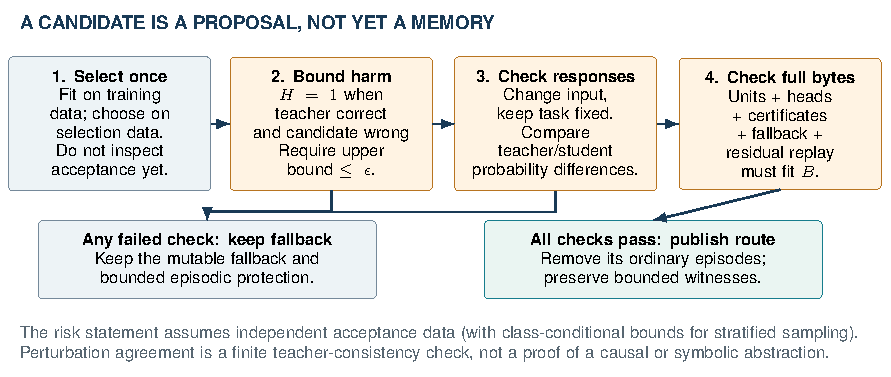
\includegraphics[width=\textwidth]{figures/03_admission.pdf}
\caption{\textbf{Operational admission, including legitimate refusal.} Selection, excess-harm uncertainty, finite perturbation agreement, and full-byte feasibility play different roles. A failure returns the task to episodic fallback. This is a policy for what to retain, not a claim that a small neural representation has become a uniquely identifiable symbolic concept.}
\label{fig:admissionapp}
\end{figure*}

\section{Acceptance Rule and Statistical Assumptions}
\label{app:bounds}
\subsection{Excess-risk interpretation}
Let $f$ and $g$ be fixed classifiers conditional on the pre-acceptance history. Define $H=1$ when $f$ is correct and $g$ is wrong. The reverse event, in which the candidate corrects a teacher error, contributes negative excess risk. Therefore
\begin{equation}
\begin{aligned}
\risk(g)-\risk(f)&=\Pr(H=1)\\
&\quad-\Pr(g\text{ correct},f\text{ wrong})\\
&\le\Pr(H=1).
\end{aligned}
\end{equation}
A harmful-disagreement bound is conservative because it does not credit candidate improvements. It is also only teacher-relative: a weak teacher can pass information to a weak student. The observed teacher-accuracy floor is a separate heuristic guard and does not turn the bound into an absolute-risk guarantee.

For independent acceptance draws, the one-sided Clopper--Pearson construction bounds the Bernoulli event probability \cite{clopper1934}. Spending $\alpha/T$ per task and testing one preselected proposal gives an at-most-$\alpha$ family-wise probability of an incorrectly bounded committed proposal under the stated assumptions. Selection can use arbitrary training computations without affecting this argument, provided neither the candidate nor its selection depends on acceptance examples.

The result does not certify the adaptive proposal search using the selection set, does not cover repeated threshold tuning after viewing acceptance outcomes, and does not carry over automatically to a shifted task distribution. If the same task is revisited for a new admission attempt, it needs a fresh independent acceptance sample or a newly specified sequential-testing procedure. The current code makes one attempt for each task ID in the stream.

\subsection{Stratified image calibration}
In Digits and CIFAR, acceptance examples are sampled separately within classes. If error probabilities differ by class, their pooled sum is not a sample of identically distributed Bernoulli trials conditional on the class counts. The code therefore forms one bound per class at failure level $\alpha/(TC)$ and weights those bounds by the evaluation class prior. A missing class contributes upper bound one. For balanced task accuracy the class weights are $1/C$.

This correction also states the calibration-data cost. With no observed harmful events, a single IID upper bound is $1-\alpha_t^{1/n}$. To make it at most $\epsilon$, one needs
\begin{equation}
n\ge\left\lceil\frac{\log\alpha_t}{\log(1-\epsilon)}\right\rceil.
\label{eq:nmin}
\end{equation}
For a uniform per-class requirement, substitute $\alpha_t/C$. This is a necessary sample count for that construction even with a perfect observed candidate, not a statement about whether a computational skill exists. The small Digits acceptance partitions can fail this requirement. The CIFAR configuration allocates 140 acceptance images per class so that admission is not impossible solely because of the zero-event sample bound at the default horizon.

If acceptance inputs are correlated frames, repeated augmentations of the same image, or repeated trials on the same raw example, counting them as independent increases confidence unjustifiably. The base examples, not the number of perturbations, determine the binomial sample count. For a correlated deployment stream, an independently sampled calibration batch or a different concentration argument is required. No temporal-mixing theorem is asserted by this prototype.

\subsection{Perturbation-response gate}
For a fixed task, the teacher and candidate each evaluate $x$ and $\tau(x)$. Responses are differences of class probabilities, so a constant logit offset does not by itself determine the score. The gate averages squared teacher--candidate response discrepancies over examples, classes, and four seeded transformations and takes the square root. The default threshold is 0.20.

Structured transformations replace one pair of synthetic operands, including the nuisance pair, while leaving the task unchanged. Image transformations attenuate one image row or globally scale intensity. No transformed ground-truth labels enter this check or the learner objective. The gate is therefore not an IIT loss or a DAS causal-variable alignment \cite{geiger2022,geiger2024}. It can reject candidates that fail to reproduce a teacher response, but the teacher response itself may be wrong or spurious. The main claim requires its incremental value over the no-response ablation.

The shuffled-response ablation permutes teacher response rows before comparison, breaking input correspondence while keeping response values. It is a corruption control, not an alternative causally meaningful teacher. The ungated arm removes competence, risk, and response-quality gates but retains the byte transaction. Its low storage or zero subsequent forgetting can coexist with poor task acquisition; all three metrics must be reported.

\section{Workloads, Access, and Reproducibility}
\label{app:data}
\subsection{Controlled task families}
For the arithmetic family, raw fields $(a,b,c,d,e,f,n_1,n_2)$ are independently standard normal. The three latent values are $(a-b)/\sqrt2$, $cd$, and $(e+f)/\sqrt2$. The initial nine instruction weights, known only to the generator, are $(1,0,0)$, $(0,1,0)$, $(0,0,1)$, $(1,1,0)$, $(0,1,1)$, $(1,0,1)$, $(1,2,1)$, $(2,1,1)$, and $(1,1,2)$. A task label is the sign of the weighted sum. The learner sees the raw fields and task ID, not these weights or latent values.

The nonlinear family uses $\tanh(a)-\tanh(b)$, $\tanh(c)\tanh(d)$, and $\sin(e+f)$ with the same task-weight scaffold. It is a second function family, not independent evidence about arbitrary input structure: both families retain paired operands and thresholded compositions. The unrelated-target control uses fresh task-specific coefficients in a trigonometric/quadratic rule. It supplies no common named primitive inventory. Independently drawn coefficients are fixed for a task across its splits.

Long-stream generators add seeded signed weight vectors after the finite initial catalog. Stress profiles run 30 tasks by default; 100-task runs require an explicit larger horizon and a byte grid that can hold the common fallback. The preallocated task-conditioned fallback grows with the declared horizon, and that cost is included for all methods. The implementation does not claim an indefinitely extensible task-ID embedding at zero cost.

\subsection{Synthetic split protocol}
Every seed and task has independently seeded train, selection, acceptance, and test arrays. Default pilot counts are 768, 128, 256, and 768, respectively. Confirmation uses 2,048 training, 512 selection, 2,048 acceptance, and 4,096 test examples. Separately seeded shifted, scaled, and primitive-essential sets are observer-only prospective evaluations. An essential subset is defined by a label change when one primitive is omitted; it must not be selected from a model's errors.

The current synthetic families have already informed development. New seeds within them are replication, not a genuinely independent task-family confirmation. The final manuscript must distinguish that limitation from a held-out family designed and frozen before parameter selection. The unrelated stream and image benchmarks supply complementary boundaries but do not erase prior tuning on arithmetic.

\subsection{Digits and CIFAR-100}
Digits uses the bundled optical-recognition dataset documented by scikit-learn \cite{digits2026}, with images flattened to 64 values and normalized from their recorded intensity range. Each consecutive class pair is one two-way task. A stratified 25\% test split is held out; the remaining examples are split into training and a 35\% calibration pool, which is divided 40/60 between selection and acceptance. Counts depend on class availability and are exported. This is neither MNIST nor ten-class class-incremental inference.

CIFAR-100 uses the original official training and test partitions \cite{krizhevsky2009}. A seed determines a 100-class order; every ten classes form one task. For each class, the first 30 shuffled training examples go to selection, the next 140 to acceptance, and the remaining 330 to training. Local task labels index the ten classes in that task; the model is supplied the task identifier. The official 100 test images per class are used only by the observer.

The supplied image encoder has two small convolutional stages, global pooling, and a compact feature projection. No pretrained weights are loaded. The runner is complete and fails explicitly on download errors, but executing it is not equivalent to a strong image-benchmark result. A matched competitive-backbone track and public modular/latent-replay implementations are pending requirements of the final evaluation. Their additional pretrained parameters, data, adaptation layers, and codec state must be disclosed and charged.

\subsection{Current versus historical data}
The fallback optimizer reads current training examples and replay records. Unit and head fitting read current training examples; candidate selection reads the selection set; one candidate receives acceptance evaluation. No old-task label service is queried, and no numerical synthetic target is used to train the backbone. Witnesses are explicit retained historical records and remain in the budget.

A main baseline reserves the same selection/acceptance partitions, making annotation budgets comparable. Since FAMP uses those labels for decisions, a stronger all-annotated-data replay condition is also needed: the baseline may train on all non-test labels, while the FAMP acceptance partition remains independent of its own optimizer. These settings must be labeled separately, rather than described as identical gradient information. An external baseline's validation protocol may require a further partition; that cost and access are recorded in its adapter manifest.

\begin{figure*}[t]
\centering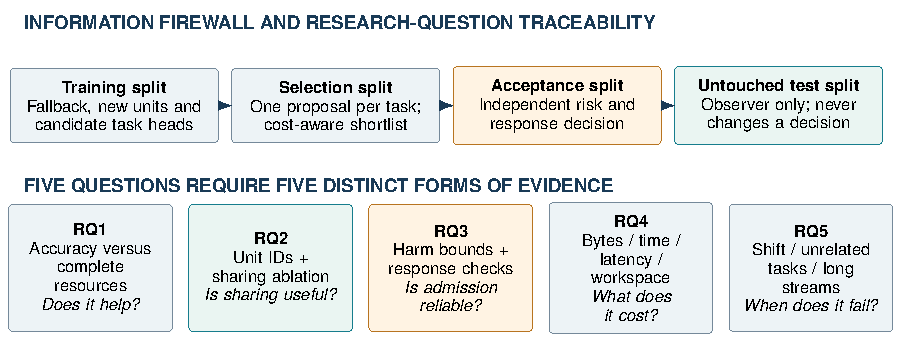
\includegraphics[width=\textwidth]{figures/04_protocol.pdf}
\caption{\textbf{Information access and claim mapping.} Training, selection, acceptance, and test serve different roles. The five research questions require different evidence: a committed unit does not establish an improved frontier, and a smaller byte count does not establish useful reuse.}
\label{fig:firewall}
\end{figure*}

\section{Frozen Hyperparameters and Baseline Obligations}
\label{app:hyper}
\begin{table*}[t]
\caption{\textbf{Configuration, not result values.} Pilot settings support implementation and failure analysis. Confirmation settings are fixed prospective configurations, not completed experiments. The source and configuration digest must accompany each populated results table.}
\label{tab:config}\centering\small
\begin{tabularx}{\textwidth}{Ylll}
\toprule
Setting & Pilot & Confirmation & Meaning\\\midrule
Seeds & 811, 823, 839 & 1009, 1013, 1019, 1021, 1031 & Independent initialization/data streams\\
Recorded orders & 0 & 0, 1, 2 & First-three-fixed curriculum variants\\
Fallback updates/task & 120 & 300 & Adam, reset at task boundaries\\
New-unit updates/task & 120 & 300 & Label + teacher-target construction\\
Head updates/proposal & 30 & 80 & Frozen-unit linear head fitting\\
Current/replay batch & 64 / up to 64 & Same & Two mean cross-entropy terms\\
Fallback/unit learning rate & 0.003 & 0.003 & No test-set search\\
Head learning rate & 0.03 & 0.03 & Adam on cached frozen features\\
Fallback hidden widths & 48, 48 & Same & Common base across primary arms\\
Unit hidden/output widths & 16 / 8 & Same & Compact executable map\\
Distillation weight / temperature & 0.5 / 2 & Same & No persistent teacher duplicate\\
Shortlist / composition width & 3 / up to 2 units & Same & Bounded recency search\\
Selection slack & 0.06 & 0.06 & Relative selection accuracy tolerance\\
Teacher-accuracy screen & 0.70 & 0.70 & Observed competence, not a bound\\
Excess-harm tolerance & 0.08 & 0.08 & Teacher-relative risk increment\\
Family failure probability & 0.05 & 0.05 & Divided by tasks; then by class if stratified\\
Response RMS threshold & 0.20 & 0.20 & Finite teacher-consistency test\\
Witnesses/task & 4 & 4 & Stored and charged\\
Replay reserve at admission & 8/unresolved task & Same & Current-boundary feasibility guard\\
Synthetic total-state caps & 24, 48 KiB & 16, 24, 32, 48, 64 KiB & Includes common fallback\\
Digits total-state caps & 48 KiB & 32, 48, 64 KiB & Conditional binary tasks\\
CIFAR runner total-state caps & Not run & 1, 2, 4 MiB & Small-backbone TIL track\\
\bottomrule
\end{tabularx}
\end{table*}

\subsection{Optimizer and presentation accounting}
The fallback draws 64 current examples with replacement per update. When replay exists, it separately draws up to 64 old examples and adds their mean cross-entropy to the current mean loss. Therefore an update can contain 128 example presentations; it is not a 64-example half-current/half-old mixture. With few retained records, all available records can be used. The number of presentations is logged, and admitted tasks can change which old data remain available.

DER++ adds a coefficient-0.5 mean-squared loss to stored float16 insertion-time logits. Its task-batch priority memory differs from the original method's general-continual-learning setting \cite{buzzega2020}; that adaptation must appear in captions and code metadata. Ordinary replay does not store logits or run an extra forward solely to construct unused logits. All arms train the same fallback even when most tasks become immutable. Candidate discovery is additional work, not an equal-update argument for equal compute.

\subsection{Internal conditions}
\texttt{er\_fp32} stores ordinary float32 episodes. \texttt{er\_comp} stores float16 structured inputs or uint8 images. \texttt{derpp} uses the packed codec and additional stored logits. \texttt{independent} builds compact units with the same gates but never reuses existing ones. \texttt{famp} enables reuse and composition. \texttt{no\_cf} removes only the response criterion. \texttt{shuffled\_cf} preserves the criterion but destroys correspondence. \texttt{ungated} bypasses quality checks while retaining the storage cap.

Two additional confirmatory ablations are specified but not executed in the pilot: disallow two-unit composition while leaving the singleton shortlist unchanged, and select a rank/width-matched independent unit instead of the shared proposal. They require distinct configuration identifiers in the table registry. A change that also changes shortlist size is not a clean composition ablation.

\subsection{External methods}
MNTDP and the compositional lifelong-learning framework are mandatory related-method comparisons because they already address reuse and allocation \cite{veniat2021,mendez2021}. REMIND, Latent Replay, and AHR are needed to compare with compressed experience rather than an artificially expensive float32 buffer \cite{hayes2020,pellegrini2019,nori2025}. PackNet and recent compact adaptation modules provide task-specific parameter-storage controls \cite{mallya2018,yildirim2026}. These methods are not implemented by relabeling the simple internal baseline.

Each public-method adapter must declare source commit, checkpoint initialization, frozen versus trainable parts, replay/codec precision, task-ID access, pretrained data, parameter count, stored optimizer state, and validation-label use. Retain original algorithms where compatible. If a strict byte cap changes eviction or growth, report both the original-budget method and the named capped adaptation. No external score is copied from a paper into a table whose data access or backbone differs.

A compute-budgeted replay run spends the proposed method's measured time on additional permitted training updates. A total-byte baseline spends the same complete cap on its own best memory representation. Those controls are essential because FAMP discovery has overhead and compact episodes may already be cheaper than neural units on small inputs. Total-budget work is established prior art \cite{seo2024}; its principles apply equally to FAMP and its comparators.

\section{Research-Question-to-Table Registry}
\label{app:registry}
\begin{table*}[t]
\caption{\textbf{Claim traceability.} Main-table identifiers refer to the manuscript. Existing pilot fields are named; measurements absent from the pilot remain explicit final-evaluation obligations. The machine-readable registry in the artifact contains these statuses.}
\label{tab:trace}\centering\small
\begin{tabularx}{\textwidth}{lYYY}
\toprule
Question & Required contrast and table & Existing code/export & Additional confirmation obligation\\\midrule
RQ1 & FAMP vs packed replay, DER++, independent units; main Table 1 & \texttt{all\_runs.csv}: accuracy, acquisition, forgetting, train time, persistent bytes & Validation-selected $B^*$; public compressed/modular baselines; independent test noninferiority\\
RQ2 & Sharing on/off and composition on/off; main Table 2 & Unit IDs, routes, \texttt{reuse\_ablation.csv}, \texttt{events.json} & Clean no-composition arm; matched independent capacity; related/unrelated streams\\
RQ3 & Full/no-CF/shuffled/ungated; main Table 3 & Acceptance harm, upper bound, teacher/candidate accuracy, response RMS, rejection reason & Fresh observer harmful-disagreement audit; calibration-size sweep; teacher-strength sweep\\
RQ4 & Complete bytes and cost; main Table 4, Appendix Table A3 & Per-stage ledger; construction time; final-state file bytes; inference microbenchmark & Isolated peak host/GPU; cold/hot batch-1/128 latency; repeated timing and supported energy counters\\
RQ5 & Shifts, essential cases, unrelated/long tasks; main Table 5 & Stress and unrelated generators; rejection and capacity logs & Explicit observer-only shift/essential runner; arbitrary-order track; long-horizon confirmation\\
\bottomrule
\end{tabularx}
\end{table*}

\subsection{Primary frontier analysis}
The main decision uses a predeclared validation accuracy target $a^*$ and tolerances $\delta_A=0.01$, $\delta_Q=0.01$, and $\delta_F=0.02$ for final accuracy, acquisition, and forgetting. For method $m$, choose the smallest actually evaluated cap whose validation result meets the target and auxiliary tolerances. Test performance is then reported once at that operating point. If none meets the requirement, label the point infeasible; do not interpolate a crossing or choose a different target after viewing test results.

The target is defined on a separate development sequence using a common full-budget reference. Since current task acceptance is not the same as method-level budget selection, these roles use different data or explicitly nested partitions. Existing pilot test points can be plotted descriptively, but do not constitute a validation-selected noninferiority frontier. This is why pilot figures are not copied into main Table 1.

The complete comparison has two tracks. A fixed-cap track reports all methods at identical total published-state caps, including their base models. A minimum-cap track reports $B^*$ at a matched competence target. Compute and inference latency remain coordinates of the outcome rather than being discarded after a favorable storage result. A frontier point is dominated if another feasible method is no worse on all declared resources and competence metrics and strictly better on at least one.

\subsection{Sharing-specific evidence}
For every unit, log its immutable parameter hash, admission task, client tasks, serialized payload, and changes in outputs when its contribution is removed. Removing a unit means zeroing its feature contribution at the already trained task head; it is not retraining a stronger replacement model. Average dependency effects first over that unit's clients and then at the seed level. A large ablation effect indicates dependence on the retained object, not identification of a semantic primitive.

The strongest reuse comparison is against independent units built with the same data, teacher, optimization budget, acceptance policy, and interface size. If both methods perform similarly, the benefit may come from freezing task-specific solutions rather than sharing. If FAMP stores fewer independent units but extra heads, certificates, or fallback episodes consume the saving, no full-state advantage has been established. These are distinct potential failures of RQ2 and RQ1.

\subsection{Admission quality}
The observer measures the probability of teacher-correct/candidate-wrong outcomes on fresh examples for both accepted and rejected proposals where a temporary candidate snapshot is available. These snapshots belong to the offline audit archive, never the learner's retained memory. If they are not saved, that observer metric is marked missing rather than reconstructed from acceptance outcomes and called independent validation.

Report task-level admission coverage, harmful-disagreement rate, response discrepancy, rejection reasons, and construction cost. For each condition, list how many proposals fail because of insufficient statistical precision rather than observed error or response mismatch. A confidence interval that does not meet a tolerance is not proof that the true error exceeds it. The image sampling mode, class counts, and class weights are part of every certificate audit.

\section{Systems Measurement Protocol}
\label{app:systems}
\subsection{Three different memory metrics}
\textbf{Published-state payload} is the exact sum in the byte ledger. \textbf{Serialized state} includes the file format's overhead, tensor names, alignment, and container metadata. \textbf{Peak working memory} measures actual host/device allocations during the learner's execution window, including optimizer moments, feature caches, gradients, candidate proposals, and temporary conversions. Report all three; a claim on one does not imply the others.

The code's reported GPU peak, when available, spans the run and can include observer evaluation. Before claiming a training-only peak, bracket the learner separately and reset the relevant allocator statistics at a synchronized boundary. Host RSS, Python allocator overhead, and pinned transfer buffers require process-level measurement rather than summing tensor sizes. For a constrained device, a method whose published state fits but whose construction cannot execute within physical RAM is infeasible.

\subsection{Time and energy}
Record total learner wall time, candidate-fitting time, serialization time, and total learning-plus-serialization time. Separate dataset acquisition and offline observer work. For steady-state timings, load inputs before the measured window only if every comparator receives the same treatment, and report cold-load time separately. Run methods in randomized order after warm-up and record CPU thread count, GPU name, library versions, synchronization points, and batch sizes.

At least three repeated timing trials per trained configuration estimate execution variability; training seeds remain the scientific replication unit for accuracy. Report median and p95 task-boundary latency because rejection or multiple proposals can create long pauses. Profile batch-1 and batch-128 inference under the empirical task-route mixture as well as route types separately. A microbenchmark only on the last task cannot characterize the full serving distribution.

Count energy only when device telemetry is supported and the interval and idle subtraction are documented. No joule estimate is inferred from runtime or a nominal board power. Report unavailable counters as missing, not zero. FLOP estimates must state whether backward passes, head fitting, teacher forwards, packing, and validation are covered; scalar derivative counts or optimizer-step counts are not FLOPs. These requirements prevent a narrow kernel saving from being mistaken for an end-to-end systems result.

\begin{table*}[t]
\caption{\textbf{Additional RQ4 systems results, intentionally empty.} All methods use the same device, thermal/power configuration, and declared measurement windows. Energy is left missing if no valid counter exists. The completed table must identify the reference artifact and profile hash.}
\label{tab:hardware}\centering\small
\begin{tabularx}{\textwidth}{Yrrrrrrr}
\toprule
Method & \shortstack{Total\\seconds} & \shortstack{Boundary\\p95 ms} & \shortstack{Host\\MiB} & \shortstack{GPU\\MiB} & \shortstack{Batch 1\\p95 ms} & \shortstack{Batch 128\\p95 ms} & Joules\\\midrule
Packed replay &\blank&\blank&\blank&\blank&\blank&\blank&\blank\\
DER++ &\blank&\blank&\blank&\blank&\blank&\blank&\blank\\
Latent replay &\blank&\blank&\blank&\blank&\blank&\blank&\blank\\
Public modular baseline &\blank&\blank&\blank&\blank&\blank&\blank&\blank\\
Independent units &\blank&\blank&\blank&\blank&\blank&\blank&\blank\\
FAMP &\blank&\blank&\blank&\blank&\blank&\blank&\blank\\
\bottomrule
\end{tabularx}
\end{table*}

\subsection{Resource-sensitive ablations}
Sweep unit hidden width 8/16/32, output width 4/8/16, witness count 0/4/16, shortlist length 1/3/8, and the construction-update budget. Change one mechanism at a time on development sequences. The zero-witness condition removes runtime regression checks but does not invalidate structural immutability; it must not be labeled a theorem-free condition. A wider shortlist changes both search opportunity and compute. A quantized-unit condition must count scales/zero points and re-run acceptance after quantization rather than reuse a float32 certificate.

A task-aware frozen-encoder replay baseline and task-specific heads may outperform a more complex unit store. Such a result is relevant, not a reason to exclude the baseline. Similarly, allowing a compressed-replay baseline to retain more examples at the same byte cap is the correct comparison, not an unfair extra-data advantage. Its stored unique observations and any pretraining remain explicitly disclosed.

\section{Failure Regimes and Boundary Tests}
\label{app:failure}
\subsection{Weak teachers and premature publication}
The system distills a learned teacher, not an oracle. Short fallback training can produce a cheap, consistent but incompetent candidate. The minimum teacher-accuracy screen partially addresses this; it does not establish that a teacher's response to irrelevant inputs is appropriate. Sweep teacher training budget and teacher competence independently where possible, and report acquisition before publication. The ungated control deliberately exposes frozen mistakes: zero later forgetting is not favorable when the route never learned the task well.

\subsection{Shift and task relatedness}
Evaluate raw-input scale changes, mean shifts, and nuisance perturbations without adapting the stored heads. A closed immutable route retains its function, not guaranteed accuracy under a new distribution. For synthetic essential cases, define the sampling criterion from the known rule and report conditional sample counts. Never select hard cases by searching for mistakes of one method.

The unrelated stream tests whether reuse admission is selective. A correct controller may allocate independent units or fall back to replay, paying search time without gaining shared structure. At increasing task counts, interfaces and witnesses grow even if units are reused. Measure the fraction of cap spent on metadata and the first stage where no new route can fit. The algorithm must continue predicting on fallback tasks and include them in all averages.

\subsection{Task identity and input interfaces}
A unit over fixed operand positions is not a position-independent arithmetic routine. Relocating operands requires a supplied or learned input adapter, whose parameters, search cost, and task metadata must be charged. This prototype does not contain that adapter. The arithmetic study therefore supports reuse over a fixed input schema, not arbitrary argument binding. Likewise, a task-conditioned classifier is not task discovery; hiding the task ID requires an additional selector that must be evaluated and budgeted.

\subsection{Candidate response consistency versus abstraction}
Teacher probability differences can be preserved by different internal implementations. Successful matching need not reveal a unique mathematical operation; failure can reflect an inaccurate teacher or an inadequate perturbation family. Formal causal-abstraction approaches require stronger commitments about variables and interventions \cite{geiger2022,geiger2024}. FAMP does not use a successful gate as proof of that stronger interpretation. The paper's algorithmic claim is useful executable sharing under resource constraints.

\section{Statistical Plan and Release Gate}
\label{app:statistics}
For accuracy differences, average repeated orders within seed, pair methods by seed, and compute a two-sided interval across independent seeds. The main three contrasts are FAMP versus packed replay, DER++, and independent units. Use simultaneous intervals for those primary comparisons; additional ablations are explicitly exploratory. With five seeds, uncertainty remains substantial, so report raw paired outcomes as well as aggregate intervals. Do not treat unit clients, task checkpoints, or counterfactuals as extra independent replications.

For the frontier, the selected budget is chosen using validation, not test outcomes. Test noninferiority compares the selected FAMP operating point with the selected baseline operating point. Report both the statistical tolerance and the engineering target reduction. A percentage-point accuracy loss and a percentage memory reduction are different quantities; a single weighted score must not conceal an unacceptable loss of task competence.

The algorithmic paper proceeds only if memory substitution provides a measured trade-off against strong baselines and the independent-unit ablation supports a benefit from sharing. If the response gate does not improve admission relative to the no-response policy, remove that performance claim while retaining the finite-check implementation description. If FAMP only beats float32 replay but not packed or latent replay, it does not establish the intended storage result. If every image proposal is rejected, report a fallback-equivalence result and search overhead, not successful image functional learning.

The draft's tables are not filled by the pilot exporter. A separate confirmation import requires protocol version, configuration/source digest, baseline identity, task-ID setting, data split description, resource window, and human approval of the measurement manifest. Unknown or unexecuted values remain empty. A public baseline adaptation is named in the table; it is not assigned the original method's title without qualification.

\section{Artifact Inventory and Execution Status}
\label{app:artifact}
The notebook embeds all Python needed for the pilot and writes readable source files before import. It saves the environment, fixed configuration, all task decisions, candidate/acceptance statistics, accuracy matrices, per-stage byte ledgers, final state dictionaries, unit-dependence ablations, and generated insight text. The loader reconstructs every state and recomputes its byte ledger and final task accuracies. These checks are not measurements of literature-level superiority.

The executed profiles contain the controlled arithmetic/nonlinear families and Digits. The stress/unrelated generators and small CIFAR task-incremental runner are implemented but their full confirmatory profiles are not presented as executed results. Public MNTDP, REMIND, AHR, competitive-backbone integration, no-composition isolation, fresh proposal-audit snapshots, and multi-device energy/latency measurements remain marked obligations in the registry. This separation prevents the completeness of a software scaffold from being confused with completion of an empirical claim.

The code archives final tensor-only checkpoints rather than arbitrary executable pickle objects. Current-task optimizer state is not included for mid-task resume. Reproducible restart uses the recorded seeds and configuration; a new execution directory avoids silently reusing stale results. Public dataset bytes are not redistributed in the Overleaf archive. Generated synthetic data are reproducible from source and seed; observers and their saved outputs are never allowed into the live learner budget.



\section{Reference Verification and AI Assistance}
The bibliography is assembled from primary publication records, author preprints, and official software/dataset documentation. Full author lists are retained; the accompanying audit states the role of each citation and whether a method is an implementation, an adaptation, or a required external comparator. Preprints are not assigned invented venues. Software access dates and the execution environment are recorded separately because they serve different purposes.

Generative AI assisted ideation, literature retrieval, code, tests, figures, manuscript drafting, and pilot interpretation. The paper contains a dedicated AI Usage Disclosure after its references. Human review of the theoretical assumptions, primary references, baseline reproductions, data licensing, scientific claims, and final results remains required. This appendix and the main PDF are research drafts with deliberately empty result cells, not a representation that the confirmatory experiments or human submission approval have already occurred.

\bibliographystyle{plainnat}\bibliography{references}
\end{document}
